\section{Entanglement and Operator Spreading in Quantum Circuits} \label{sec:circuits}

\subsection{Entanglement Entropy} \label{sub:intro}\emph{}

Quantum entanglement describes aspects of branches of physics from high energy and quantum information theory to experimental studies of cold atomic gases. Although entanglement is so widely studied, its dynamics are less well understood. The dynamics of the entanglement entropy are closely related to the speed at which information travels or spreads. 
%One way to study this topic is to consider entanglement dynamics of spin chains. 

Entanglement entropy provides one way to quantify the entanglement and is defined as follows. For a system $AB$ divisible into subsystems $A$ and $B$, the reduced density matrices $\rho_A$ and $\rho_B$ are the full density matrix $\rho_{AB}$ traced over subsystem $B$ and $A$, respectively. If the full system is in a pure state, the $n$th Renyi entropy of density matrix $\rho$ is 
\begin{align}
S_n = \th{1-n}\log\left(\Tr\rho^n\right). \label{eqn:renyi}
\end{align}
In the limit $n\to1$ this becomes the von Neumann entropy
\begin{align}
S_{vN} = -\Tr\rho\log\rho,
\end{align}
the analogue of the classical Shannon entropy. These entropies are maximized by maximally mixed states, with entropy $N\log q$ for $N$-site systems with $q$-dimensional Hilbert spaces at each site.

Introduce entropy bounds here.

References~\cite{Keyserlingk, Jonay} discuss the speed of entanglement in brickwork models using related concepts called out of time order commutator (OTOC) and operator density. Reference~\cite{Zhou2017} quantifies the scrambling using the operator entanglement entropy opEE of the time evolution operator.

\subsubsection{Entropy Constraints} \emph{ }\label{subsub:constraints}

The following description is largely taken from~\cite{Nahum2017}. Consider a spin chain of N sites with dimension $q$. $q=2$ corresponds to spin-$\half$ particles, $q=3$ corresponds to spin-1 particles, etc. Sites are labeled by $i=1,\dots N$, while the bonds between sites are labeled by $x = 1,\dots N-1$. After cutting the system at bond $x$, define the entropy across this cut as the bipartite entanglement entropy of all sites to the right of $x$. If the whole chain is in a pure state, this is equal to the bipartite entanglement entropy of all sites to the left of $x$.

The von Neumann entropy at cut $x$ is
\begin{align}
S(x) = \-\Tr\rho_x\log\rho_x, \label{eqn:vonneu}
\end{align}
where $\rho_x$ is the density matrix of the system with all sites left of $x$ traced out, and for convenience logarithms are taken base $q$. Classically, for an arbitrary system decomposable into subsystems $A$ and $B$, the entropies satisfy $\max(S(A), S(B)) \leq S(AB)\leq S(A) + S(B)$. In quantum mechanics, this is replaced by the subadditivity of the von Neumann entropy 
\begin{align}
\left|S(A)-S(B)\right| \leq S(AB)\leq S(A) + S(B). \label{eqn:subadd}
\end{align}
If we take subsystem $A$ to be the single site between cuts $x$ and $x+1$ and subsystem $B$ to be all sites right of $x+1$, this becomes
\begin{align}
\left|S_1 - S(x+1)\right| \leq S(x) \leq S_1 + S(x+1),
\end{align}
where $S_1$ denotes the entropy of the single site between cuts $x$ and $x+1$. After some rearranging this can be written $\left|S(x+1) - S(x)\right| \leq S_1$. However, since the single site is $q$ dimensional, $S_1 \leq \log q = 1$, explaining the use of $q$ for the base. The preceding arguments taken together give the constraint
\begin{align}
\left|S(x+1) - S(x)\right| \leq 1. \label{eqn:offbyone}
\end{align}

\subsection{Circuit Architectures} \emph{}\label{sub:arch}

Instead of evolving the spin chains with Hamiltonians, this paper focuses on quantum circuits, which consist of a series of unitary operators, called gates. Simple gates act on the product of Hilbert spaces at adjacent sites. References~\cite{Keyserlingk} and~\cite{Nahum2017} both discuss circuits of this type. Both discuss random circuits, although with different sources of randomness. One source is the unitary operator chosen at each site at each time. Different gates result in different architectures. 
%If the Hilbert space at each site is $q$ dimensional, the space of 2-site unitary matrices is $q^2\times q^2$ dimensional\footnote{wrong}. To find representative behavior, each circuit is made by drawing gates from the Haar distribution. The circuits can then be averaged over these choices. 

Another source of randomness is the placement of the gates. The ``brickwork" model~\cite{Keyserlingk} uses a deterministic architecture, in which at odd times there is a gate to the right of every odd site, while for even times there is a gate to the right of every even site. The ``random" architecture~\cite{Nahum2017} chooses a random site for a single gate at each time step. This placement is then averaged over.



\subsubsection{Deterministic Limit} \emph{} \label{subsub:determ}

An interesting limit occurs when the dimensionality of each site is taken to be large. With large $q$, after a gate acts on sites $i$ and $i+1$ each site will individually saturate entropy bound in equation~\ref{eqn:offbyone}. This means that after a gate acts on bond $x$ the updated entropy will be 
\begin{align}
S(x) = \min\left\lbrace S(x-1), S(x+1)\right\rbrace + 1.\label{eqn:update}
\end{align}
This equation comes from and is proved in~\cite{Nahum2017}.

One interesting effect of the deterministic behavior is that both the butterfly velocity and the entanglement velocity approach the light cone velocity, as defined in~\cite{Keyserlingk}, which uses a brickwork circuit. The butterfly velocity is $v_B = \frac{q^2-1}{q^2+1} \to 1$ as $q\to \infty$ while the entanglement velocity is 
\begin{align}
v_E = \frac{\log\frac{q+q^{-1}}{2}}{\log q},
\end{align}
which also goes to 1 for high $q$. In this architecture all\footnote{Why is this incorrect?} information moves at the light speed because at every time step any information is maximally transported one step to the right or left. For this reason this thesis focuses on the random architecture.

\subsubsection{Surface Growth Picture} \emph{} \label{subsub:surfgrowth}

A model for the entropy growth described above is the Tetris-like surface growth picture. Here, the entropy is represented by a piecewise-constant function with the height given by the entropy across each cut, as in figure~\ref{fig:tetris}, taken from \cite{Nahum2017}. 
\begin{figure}
	\centering
	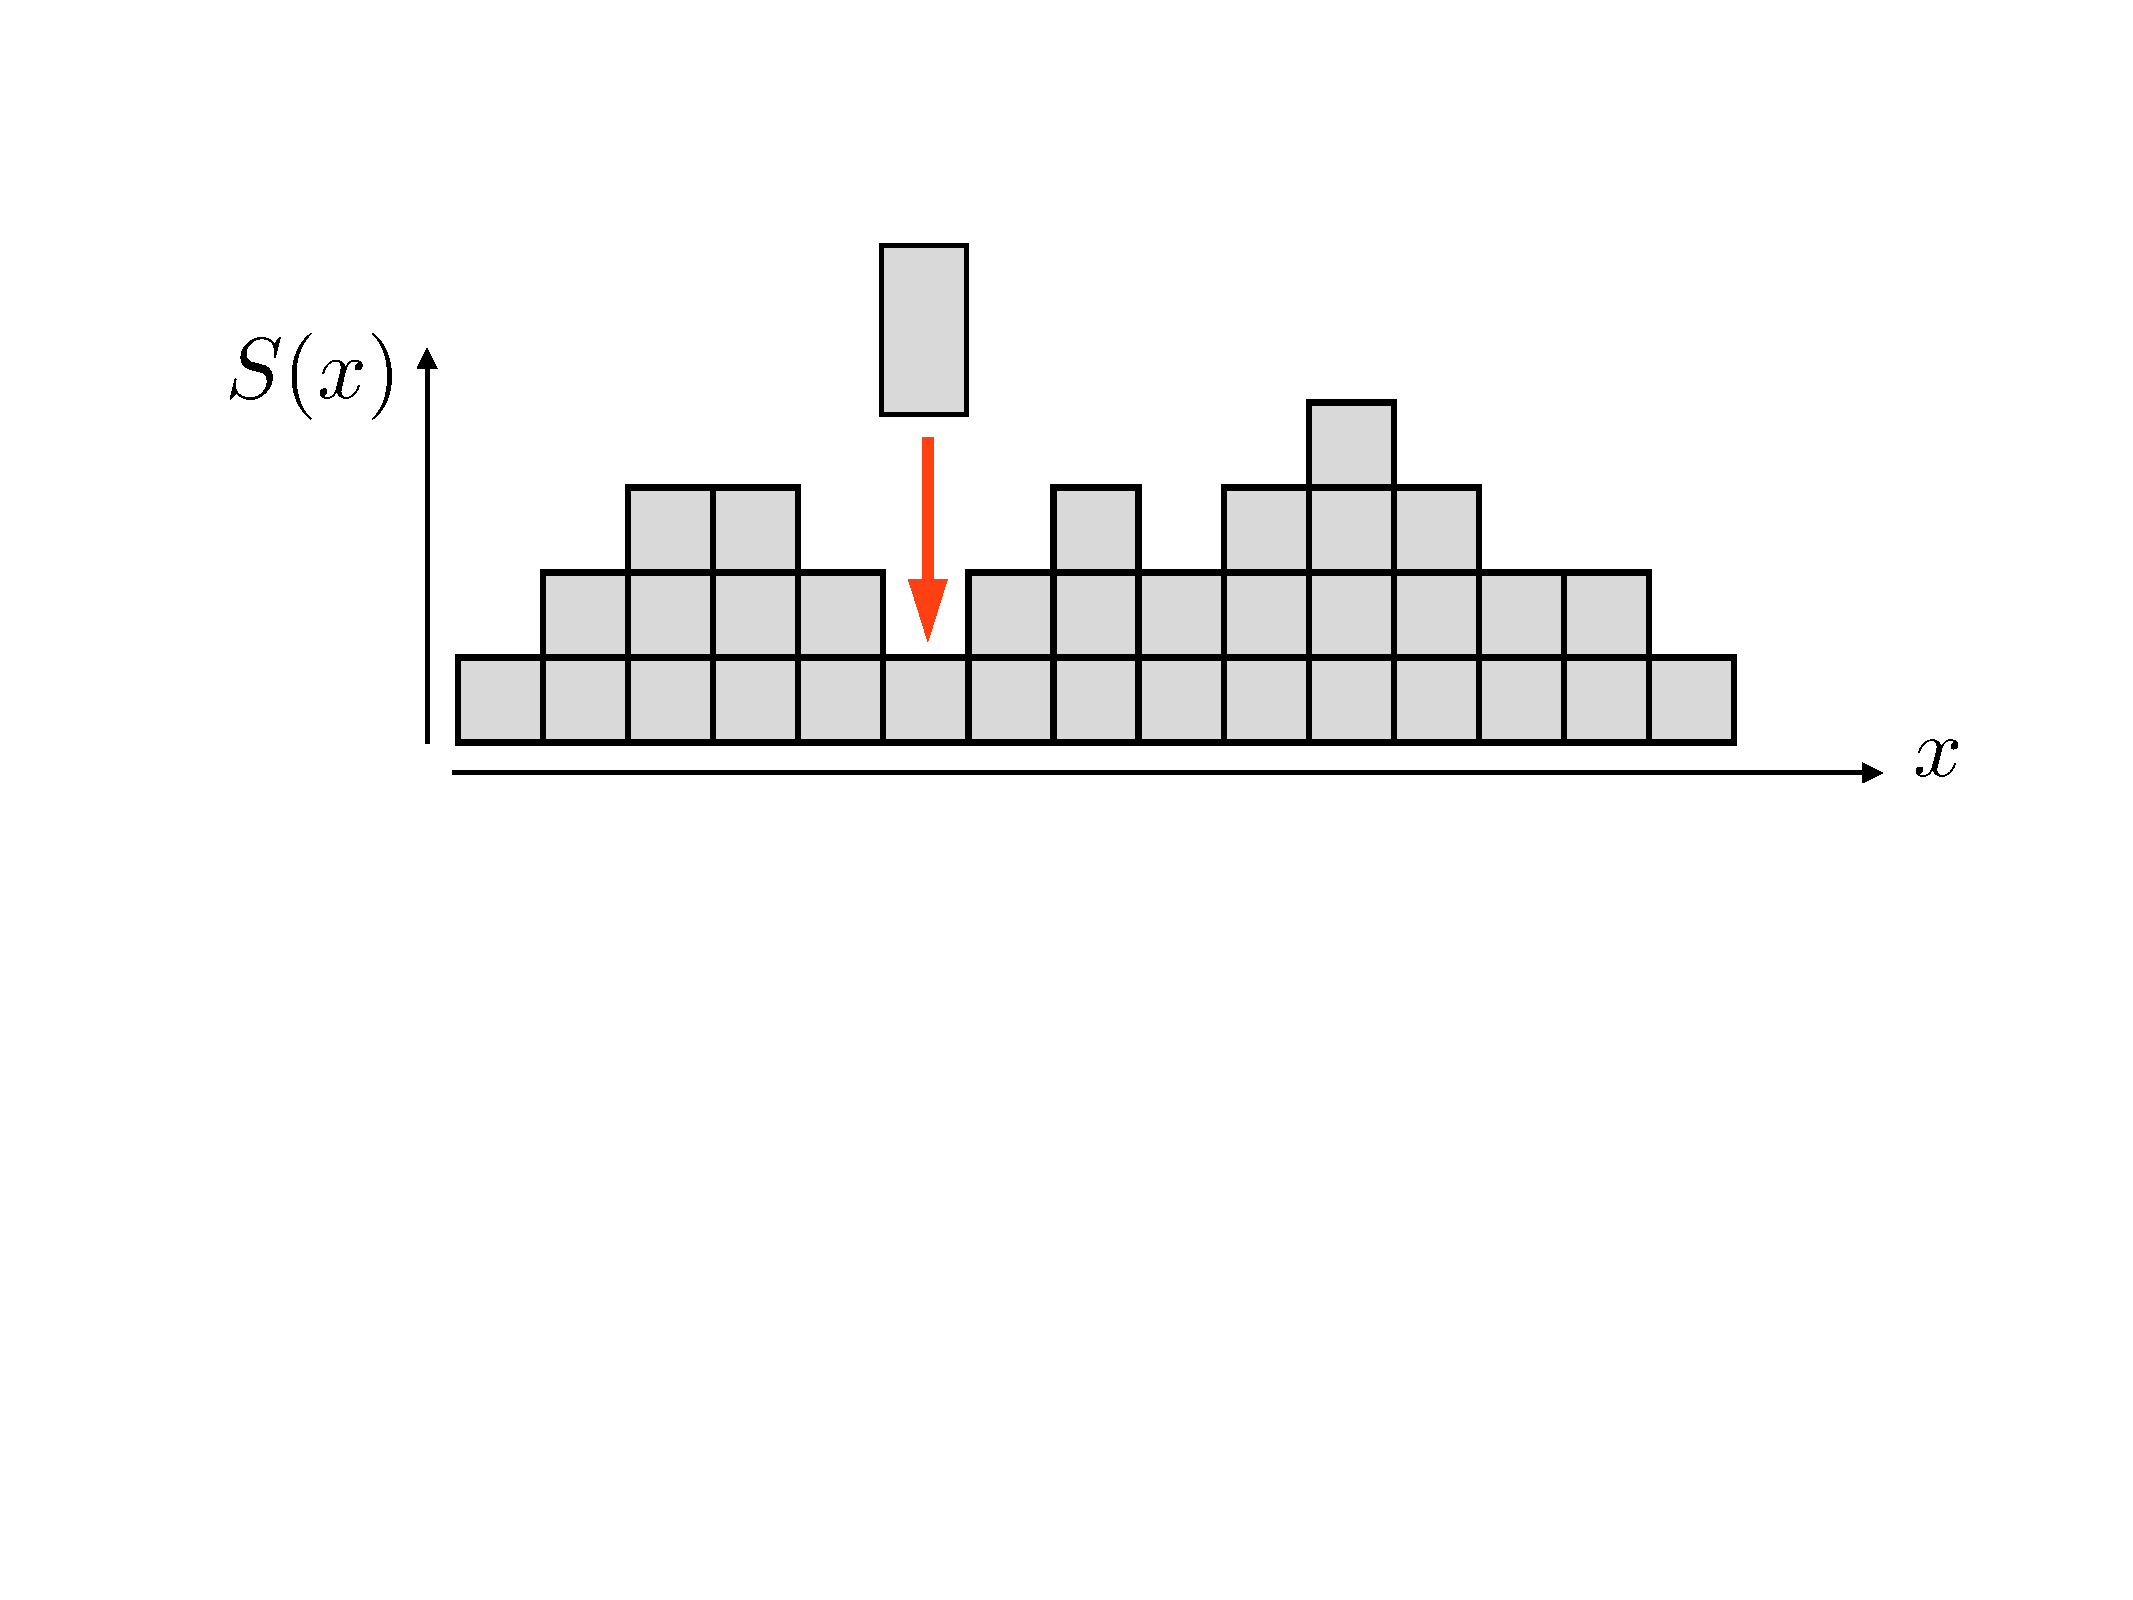
\includegraphics[width=.5\textwidth]{tetris.pdf}
	\caption{\textbf{Tetris-like model for large-$q$ chain.} The gate at cut $x$ adds enough entropy so that $S(x)$ is one greater than either of its neighbors. Figure from~\cite{Nahum2017}.}
	\label{fig:tetris}
\end{figure}
In general, it is possible for the entropy across two adjacent cuts to be equal. However, figure~\ref{fig:applyingUnitary}, also from~\cite{Nahum2017}, shows that flat sections can be destroyed but not created. 
\begin{figure}
	\centering
	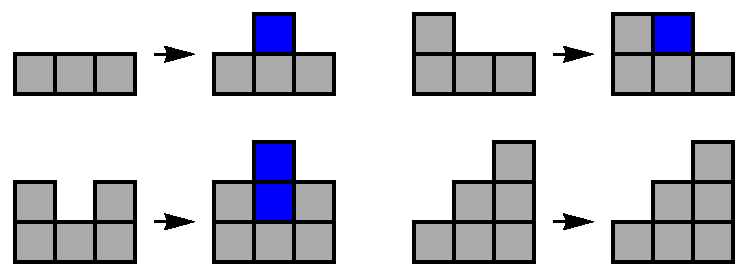
\includegraphics[width=.5\textwidth]{applyingUnitary.pdf}
	\caption{\textbf{Several possibilities for local changes} in the large $q$ model. If three adjacent cuts all have equal entropy, the two flat sections annihilate each other. There is no way to generate flat sections.}
	\label{fig:applyingUnitary}
\end{figure}

It makes sense then to only consider states that have no flat sections, so that $S(x) = S(x-1)\pm1$ for all $x$. In this case, instead of a picture like figure~\ref{fig:tetris} it is possible to represent the entropy at each bond as a point, with a diagonal slope connecting bonds. The slope will always be $\pm1$. Instead of $2\times1$ or $1\times1$ rectangles, the gates are then squares coming down point-first, as in figure~\ref{fig:diaggate}. 
\begin{figure}
	\centering
	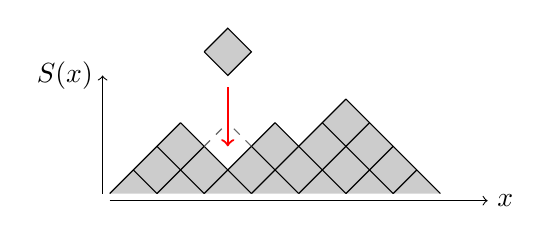
\begin{tikzpicture}[scale = .3]
\draw[->] (0, -.3) -- (16,-.3) node[right]{$x$};
\draw[->] (-.3,0) -- (-.3,5) node[left]{$S(x)$};
\fill[black!20] (0,0) -- (3,3) -- (5,1) -- (7,3) -- (8,2) --
				(10,4) -- (14,0) ;
\draw (0,0) -- (3,3);
\draw (2,0) -- (4,2);
\draw (4,0) -- (7,3);
\draw (6,0) -- (10,4);
\draw (8,0) -- (11,3);
\draw (10,0) -- (12,2);
\draw (12,0) -- (13,1);
\draw (2,0) -- (1,1);
\draw (4,0) -- (2,2);
\draw (6,0) -- (3,3);
\draw (8,0) -- (6,2);
\draw (10,0) -- (7,3);
\draw (12,0) -- (9,3);
\draw (14,0) -- (10,4);
\draw[dashed, black!60]  (4,2) -- (5,3);
\draw[dashed, black!60]  (6,2) -- (5,3);

\draw[fill=black!20] (4,6) -- (5,5) -- (6,6) -- (5,7) -- (4,6);
\draw[thick, ->, red] (5,4.5) -- (5,2);
\end{tikzpicture}
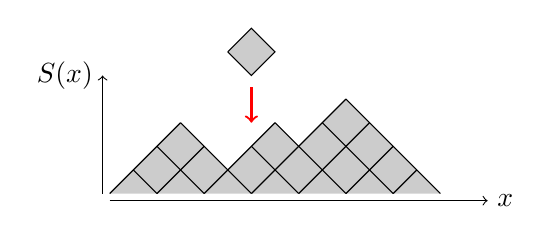
\begin{tikzpicture}[scale = .3, cross/.style={path picture={ 
		\draw[black]
		(path picture bounding box.south east) -- (path picture bounding box.north west) (path picture bounding box.south west) -- (path picture bounding box.north east);
}}]

\draw[->] (0, -.3) -- (16,-.3) node[right]{$x$};
\draw[->] (-.3,0) -- (-.3,5) node[left]{$S(x)$};
\fill[black!20] (0,0) -- (3,3) -- (5,1) -- (7,3) -- (8,2) --
(10,4) -- (14,0) ;
\draw (0,0) -- (3,3);
\draw (2,0) -- (4,2);
\draw (4,0) -- (7,3);
\draw (6,0) -- (10,4);
\draw (8,0) -- (11,3);
\draw (10,0) -- (12,2);
\draw (12,0) -- (13,1);
\draw (2,0) -- (1,1);
\draw (4,0) -- (2,2);
\draw (6,0) -- (3,3);
\draw (8,0) -- (6,2);
\draw (10,0) -- (7,3);
\draw (12,0) -- (9,3);
\draw (14,0) -- (10,4);
%\draw[dashed, black!60]  (5,3) -- (6,4);
%\draw[dashed, black!60]  (7,3) -- (6,4);
%\draw[dashed, black!60]  (6,2) -- (5,3);

\draw[fill=black!20] (5,6) -- (6,5) -- (7,6) -- (6,7) -- (5,6);
\draw[thick, ->, red] (6,4.5) -- (6,3);
%\node [draw,circle,cross,minimum width=1](B) at (6,3.5){}; 
\end{tikzpicture}

	\caption{\textbf{Another picture of the configuration in figure~\ref{fig:tetris}}. Here the cut positions are top or bottom vertices of the squares. On the left, the gate at time $t$ results in entropy growth at $x$ because at time $t-1$, $S(x-1) > S(x) < S(x+1)$. On the right the gate has no effect. Although $S(x) < S(x+1)$, the case $S(x) < S(x-1)$ is not satisfied. }
	\label{fig:diaggate}
\end{figure}
If the gate falls on a local minimum, it lifts the entropy at that bond. If the gate falls on a local maximum or a non-extremal it has no effect.